% ELEC 475 - Lab 2
\documentclass[12pt]{article}
% PACKAGES
\usepackage{graphicx}
\usepackage{tikz}
\usepackage{listings}
\usepackage{xcolor}
\usepackage{verbatim}
\usepackage{appendix}
\usepackage{amsmath}
\usepackage{xcolor}
\usepackage[colorlinks=true,
            linkcolor=blue!70!black,
            citecolor=blue!70!black,
            urlcolor=blue!70!black]{hyperref}

\usepackage{hyperref}
\usepackage{cleveref}
\usepackage{float}
\usepackage{booktabs}

% SETUP
\bibliographystyle{IEEEtran}

\definecolor{codegreen}{rgb}{0,0.6,0}
\definecolor{codegray}{rgb}{0.5,0.5,0.5}
\definecolor{codepurple}{rgb}{0.58,0,0.82}
\definecolor{backcolour}{rgb}{0.95,0.95,0.92}

\lstdefinestyle{mystyle}{
    backgroundcolor=\color{backcolour},   
    commentstyle=\color{codegreen},
    keywordstyle=\color{magenta},
    numberstyle=\tiny\color{codegray},
    stringstyle=\color{codepurple},
    basicstyle=\ttfamily\footnotesize,
    breakatwhitespace=false,         
    breaklines=true,                 
    captionpos=b,                    
    keepspaces=true,                 
    numbers=left,                    
    numbersep=5pt,                  
    showspaces=false,                
    showstringspaces=false,
    showtabs=false,                  
    tabsize=2
}

\lstset{style=mystyle}

\begin{document}
\input{titelsida}
\newpage

\providecommand{\shape}[3]{$#1{\times}#2{\times}#3$}
\providecommand{\wfig}{0.88\linewidth}

%==============================================================
\section{Architectural Specifications}
%==============================================================

All four models take a $3{\times}64{\times}64$ colour image as input. After each layer, the size of the output is
$N_{out} = \lfloor (N_{in} - K + 2P)/S \rfloor + 1$, where $K$ is the kernel size, $P$ the padding and $S$ the stride.
We also worked out the receptive field (RF) of each layer, which is the number of input pixels that can affect one
output value. It is found with $r_l = r_{l-1} + (k_l - 1)\,j_{l-1}$ and $j_l = s_l\, j_{l-1}$, starting from
$r_0 = 1$ and $j_0 = 1$.

\subsection{Base LeNet-5}

The base LeNet-5 has two convolution--Tanh--average pooling stages followed by three linear layers
(Table~\ref{tab:lenet}). The convolutions use no padding, so the maps get smaller at every step and
$16 \times 13 \times 13 = 2{,}704$ values go into the first linear layer.

\begin{table}[H]
\centering
\caption{Base LeNet-5 layers (Tanh activations; 338{,}486 parameters).}
\label{tab:lenet}
\resizebox{\linewidth}{!}{%
\begin{tabular}{llrrr}
\toprule
Layer & Output shape & Params & RF & Calculation \\
\midrule
Conv $5{\times}5$, 6, $s{=}1$, $p{=}0$ & \shape{6}{60}{60}  & 456     & 5  & $(64-5)/1+1=60$ \\
AvgPool $2{\times}2$, $s{=}2$          & \shape{6}{30}{30}  & 0       & 6  & $(60-2)/2+1=30$ \\
Conv $5{\times}5$, 16, $s{=}1$, $p{=}0$& \shape{16}{26}{26} & 2{,}416 & 14 & $(30-5)/1+1=26$ \\
AvgPool $2{\times}2$, $s{=}2$          & \shape{16}{13}{13} & 0       & 16 & $(26-2)/2+1=13$ \\
Flatten                                & 2{,}704            & 0       & -- & $16\cdot13\cdot13$ \\
Linear 2704$\to$120                    & 120                & 324{,}600 & -- & \\
Linear 120$\to$84                      & 84                 & 10{,}164  & -- & \\
Linear 84$\to$10                       & 10                 & 850       & -- & \\
\bottomrule
\end{tabular}}
\end{table}

\subsection{Modernized LeNet}

The modernized LeNet has the same layout with two changes: ReLU replaces Tanh, and $3{\times}3$ max pooling with
stride 2 replaces $2{\times}2$ average pooling. Because the stride (2) is smaller than the kernel size (3), the pooling
windows overlap. The convolutions use padding 2, so the size only shrinks in the pooling layers
(Table~\ref{tab:lenetm}), and $16\times15\times15 = 3{,}600$ values go into the first linear layer.

\begin{table}[H]
\centering
\caption{Modernized LeNet layers (ReLU, overlapping max pooling; 446{,}006 parameters).}
\label{tab:lenetm}
\resizebox{\linewidth}{!}{%
\begin{tabular}{llrrr}
\toprule
Layer & Output shape & Params & RF & Calculation \\
\midrule
Conv $5{\times}5$, 6, $s{=}1$, $p{=}2$   & \shape{6}{64}{64}  & 456       & 5  & $(64-5+4)/1+1=64$ \\
MaxPool $3{\times}3$, $s{=}2$            & \shape{6}{31}{31}  & 0         & 7  & $\lfloor(64-3)/2\rfloor+1=31$ \\
Conv $5{\times}5$, 16, $s{=}1$, $p{=}2$  & \shape{16}{31}{31} & 2{,}416   & 15 & $(31-5+4)/1+1=31$ \\
MaxPool $3{\times}3$, $s{=}2$            & \shape{16}{15}{15} & 0         & 19 & $\lfloor(31-3)/2\rfloor+1=15$ \\
Flatten                                  & 3{,}600            & 0         & -- & $16\cdot15\cdot15$ \\
Linear 3600$\to$120                      & 120                & 432{,}120 & -- & \\
Linear 120$\to$84                        & 84                 & 10{,}164  & -- & \\
Linear 84$\to$10                         & 10                 & 850       & -- & \\
\bottomrule
\end{tabular}}
\end{table}

Almost all of the parameters are in the first linear layer (324{,}600 of 338{,}486 in the base model and
432{,}120 of 446{,}006 in the modernized one). The bigger flattened input is the reason the modernized model has
about 32\% more parameters.

\subsection{AlexNet-64}

AlexNet-64 has five convolution stages for $64{\times}64$ input (Table~\ref{tab:alex}). The first convolution is
$5{\times}5$ with stride 2, max pooling ($3{\times}3$, stride 2) comes after stages 1, 2 and 5, and the classifier is
$2304\to1024\to1024\to C$ with dropout ($p{=}0.5$). The normalization layer after each convolution can be set to
none, LRN or BatchNorm2d. In the LRN version, LRN (size 5, $\alpha{=}10^{-4}$, $\beta{=}0.75$, $k{=}2$) is only used
after stages 1 and 2, like in the original 2012 network. In the BN version every convolution is followed by
BatchNorm2d.

\begin{table}[H]
\centering
\caption{AlexNet-64 layers (BatchNorm version; 6{,}611{,}402 parameters, or 6{,}608{,}842 without BatchNorm).}
\label{tab:alex}
\resizebox{\linewidth}{!}{%
\begin{tabular}{llrrr}
\toprule
Layer & Output shape & Params (conv + BN) & RF & Calculation \\
\midrule
Conv $5{\times}5$, 64, $s{=}2$, $p{=}2$   & \shape{64}{32}{32}  & 4{,}864 + 128       & 5  & $(64-5+4)/2+1=32$ \\
MaxPool $3{\times}3$, $s{=}2$             & \shape{64}{15}{15}  & 0                   & 9  & $\lfloor(32-3)/2\rfloor+1=15$ \\
Conv $5{\times}5$, 192, $s{=}1$, $p{=}2$  & \shape{192}{15}{15} & 307{,}392 + 384     & 25 & same size \\
MaxPool $3{\times}3$, $s{=}2$             & \shape{192}{7}{7}   & 0                   & 33 & $\lfloor(15-3)/2\rfloor+1=7$ \\
Conv $3{\times}3$, 384, $s{=}1$, $p{=}1$  & \shape{384}{7}{7}   & 663{,}936 + 768     & 49 & same size \\
Conv $3{\times}3$, 384, $s{=}1$, $p{=}1$  & \shape{384}{7}{7}   & 1{,}327{,}488 + 768 & 65 & same size \\
Conv $3{\times}3$, 256, $s{=}1$, $p{=}1$  & \shape{256}{7}{7}   & 884{,}992 + 512     & 81 & same size \\
MaxPool $3{\times}3$, $s{=}2$             & \shape{256}{3}{3}   & 0                   & 97 & $\lfloor(7-3)/2\rfloor+1=3$ \\
Flatten                                   & 2{,}304             & 0                   & -- & $256\cdot3\cdot3$ \\
Dropout, Linear 2304$\to$1024             & 1{,}024             & 2{,}360{,}320       & -- & \\
Dropout, Linear 1024$\to$1024             & 1{,}024             & 1{,}049{,}600       & -- & \\
Linear 1024$\to$10                        & 10                  & 10{,}250            & -- & \\
\bottomrule
\end{tabular}}
\end{table}

The last receptive field is 97 pixels, which is bigger than the 64-pixel input, so the last convolution layer can
see the whole image. The three linear layers have 3{,}420{,}170 of the 6{,}611{,}402 parameters (about 52\%) and the
five convolutions have 3{,}188{,}672.

\subsection{PyTorch Model Zoo AlexNet}

For the Model Zoo baseline we used the \texttt{torchvision} AlexNet and replaced its last layer with a
$4096\to C$ layer, which gives 57{,}044{,}810 parameters for $C{=}10$ (Table~\ref{tab:zoo}). This network was designed
for $224{\times}224$ images. With a $64{\times}64$ input, its convolution part ends with a $256{\times}1{\times}1$ map
(the first convolution is $11{\times}11$ with stride 4, so $\lfloor(64-11+4)/4\rfloor+1=15$, and the pooling layers
give $7\to3\to1$). \texttt{AdaptiveAvgPool2d((6,6))} then copies this map up to $256{\times}6{\times}6 = 9{,}216$
values. The first linear layer therefore has $9216\times4096+4096 = 37{,}752{,}832$ parameters, about 66\% of the model,
and the whole model is about nine times bigger than AlexNet-64.

\begin{table}[H]
\centering
\caption{Model Zoo AlexNet parameters ($C{=}10$).}
\label{tab:zoo}
\begin{tabular}{lr}
\toprule
Layer & Params \\
\midrule
Conv1 $11{\times}11$, 64          & 23{,}296 \\
Conv2 $5{\times}5$, 192           & 307{,}392 \\
Conv3 $3{\times}3$, 384           & 663{,}936 \\
Conv4 $3{\times}3$, 256           & 884{,}992 \\
Conv5 $3{\times}3$, 256           & 590{,}080 \\
Linear 9216$\to$4096              & 37{,}752{,}832 \\
Linear 4096$\to$4096              & 16{,}781{,}312 \\
Linear 4096$\to$10                & 40{,}970 \\
\midrule
Total                             & 57{,}044{,}810 \\
\bottomrule
\end{tabular}
\end{table}

%==============================================================
\section{Experimental Setup}\label{sec:setup}
%==============================================================

All models used Adam with a learning rate of $10^{-3}$, cross-entropy loss, batch size 128 and seed 42, unless a
different value is given. CIFAR-10 images are $32{\times}32$, so they are resized to $64{\times}64$. Tiny ImageNet-200
images are already $64{\times}64$. We normalized the inputs with the channel means and standard deviations of each
dataset from \texttt{utils/eda.py}. All the accuracies in this report are from the epoch with the best validation
accuracy. Macro-$F_1$ is the average of the $F_1$ scores of the individual classes.

The two LeNets were trained for 5 epochs on a CPU. The AlexNet versions were trained on a Tesla T4 GPU (Google
Colab) for 10 epochs in the normalization study and 15 epochs in the augmentation study. On Tiny ImageNet we trained
AlexNet-64 and the Zoo AlexNet for 10 epochs and the two LeNets for 5 epochs, on the same T4 and with augmentation.
When augmentation is on, each training image gets a random crop (4 pixels of reflect padding), a random horizontal
flip ($p{=}0.5$) and colour jitter (brightness, contrast and saturation 0.2).

The accuracy curves that \texttt{train.py} draws for Tiny ImageNet use the training images as the ``validation'' set.
For this reason we measured the saved Tiny ImageNet models again on the 10{,}000 official validation images
(\texttt{eval\_tiny\_heldout.py}), and the Tiny ImageNet scores in the tables come from that.

Figure~\ref{fig:eda} shows the class balance and the colour histograms of the two datasets. Both are perfectly
balanced (imbalance ratio 1.00), so accuracy is a safe metric, and we also report Macro-$F_1$.

\begin{figure}[H]
\centering
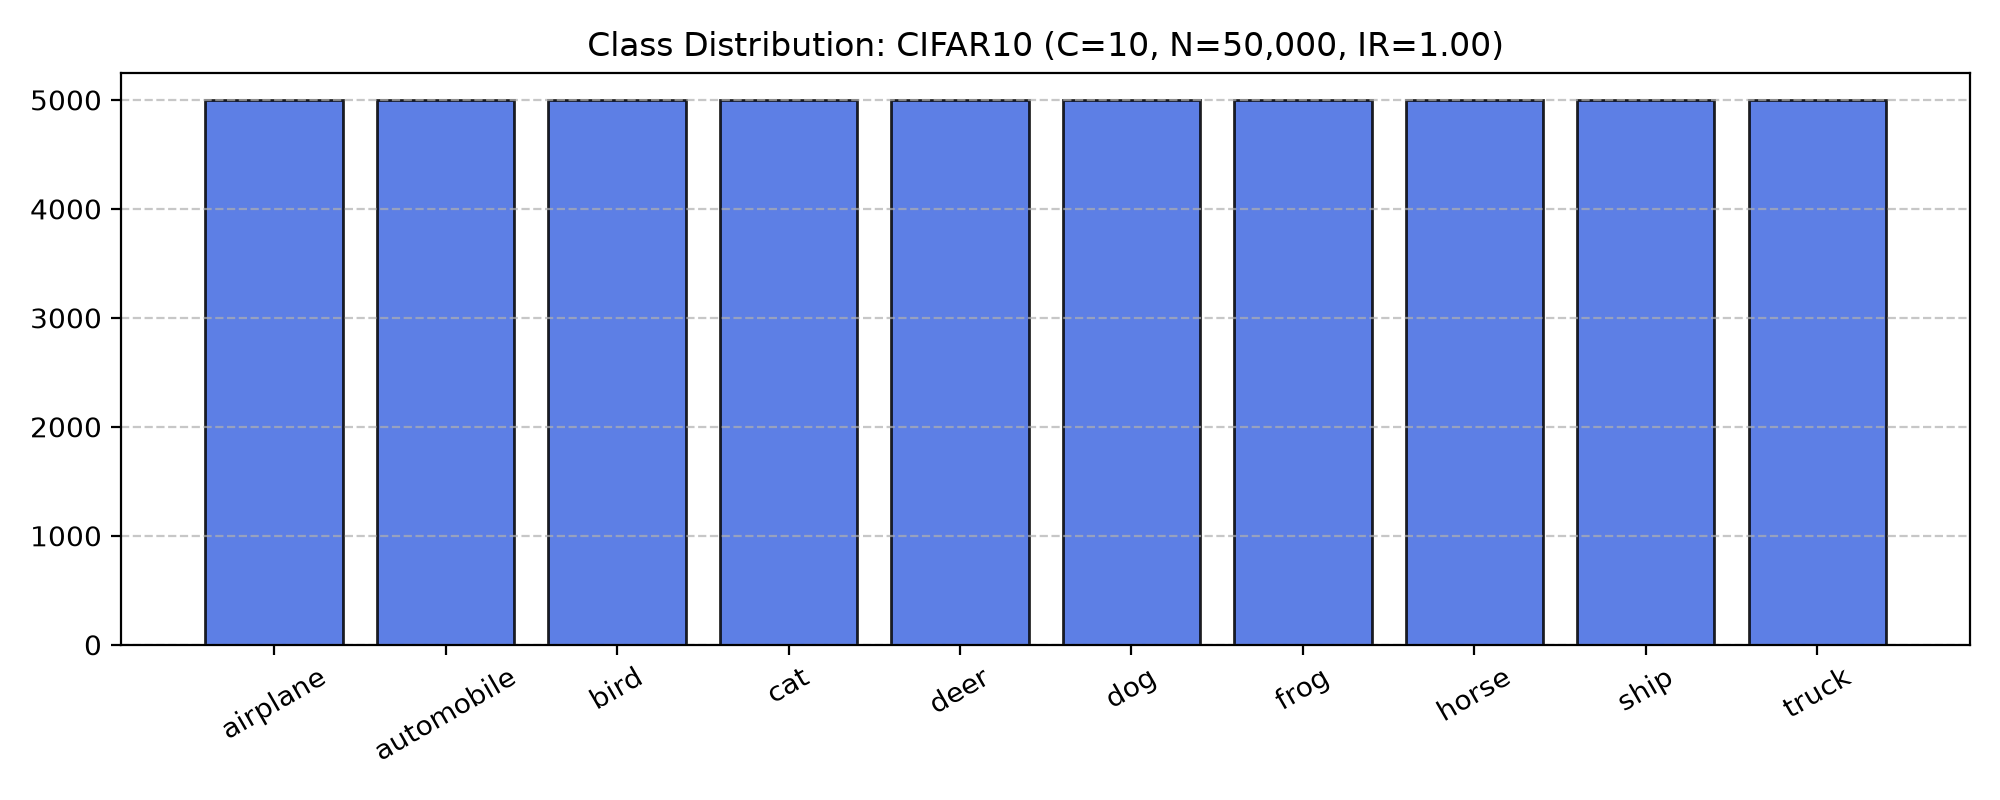
\includegraphics[width=0.48\linewidth]{plots/eda_cifar10_class_distribution.png}\hfill
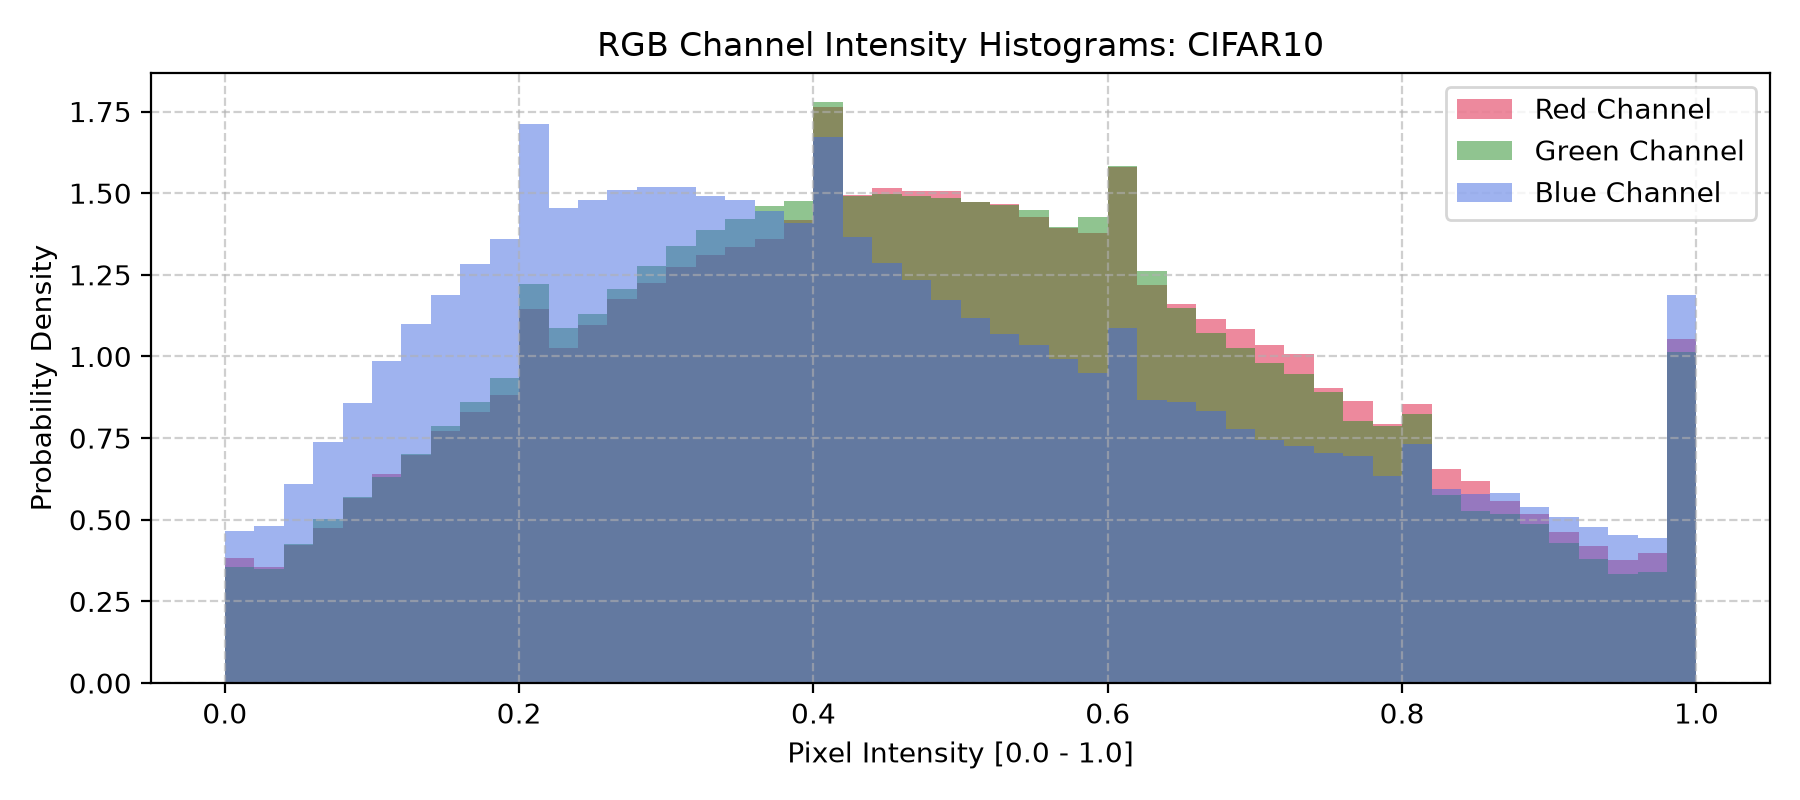
\includegraphics[width=0.48\linewidth]{plots/eda_cifar10_channel_histograms.png}\\[4pt]
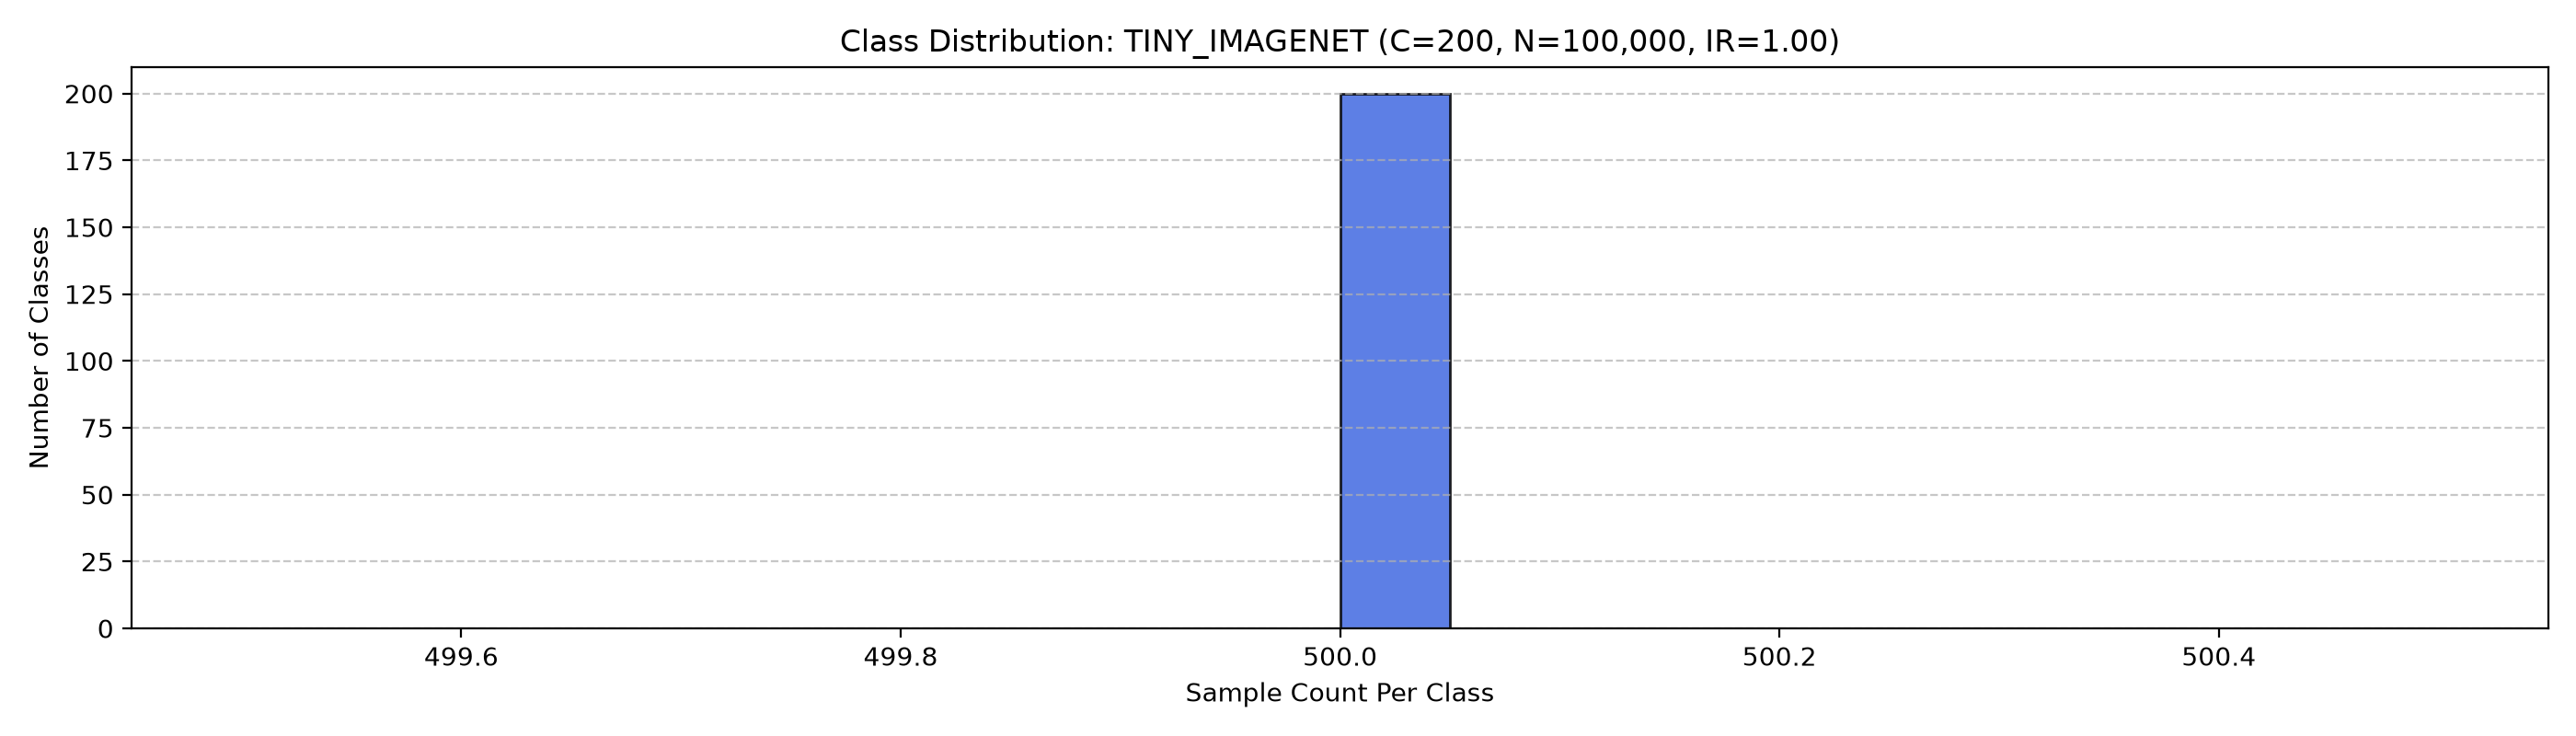
\includegraphics[width=0.48\linewidth]{plots/eda_tiny_imagenet_class_distribution.png}\hfill
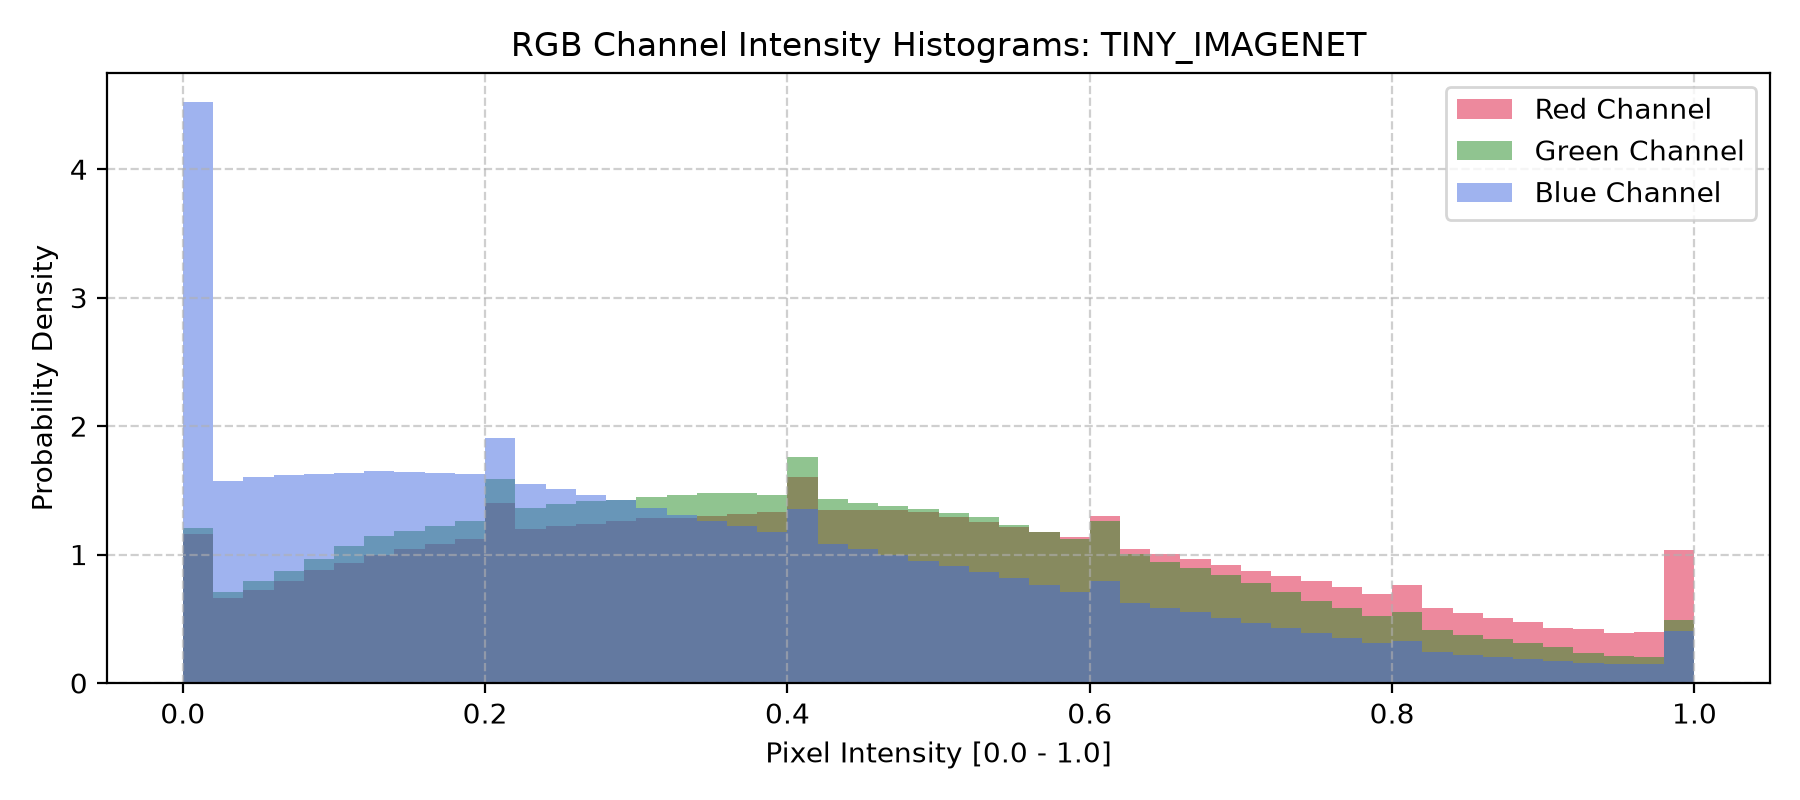
\includegraphics[width=0.48\linewidth]{plots/eda_tiny_imagenet_channel_histograms.png}
\caption{Class balance (left) and colour histograms (right) from \texttt{utils/eda.py} for CIFAR-10 (top) and
Tiny ImageNet-200 (bottom).}
\label{fig:eda}
\end{figure}

The output of \texttt{demo\_transforms.py} is shown below. It lists the data type, shape and memory location of the
image after each of the three pipelines, and the time to process 1{,}000 images.

\begin{lstlisting}[numbers=none,basicstyle=\ttfamily\scriptsize]
[1] OpenCV (cv2) Output:
    - Object Type      : <class 'numpy.ndarray'>
    - Data Type (dtype): float32
    - Shape (Layout)   : (64, 64, 3)  --> [Height, Width, Channels] (Channels-Last)
    - Value Range      : Min = 0.0000, Max = 1.0000
    - Color Space      : Converted BGR -> RGB
    - Memory Location  : Host System RAM (CPU)

[2] NumPy Output:
    - Object Type      : <class 'numpy.ndarray'>
    - Data Type (dtype): float32
    - Shape (Layout)   : (64, 64, 3)  --> [Height, Width, Channels] (Channels-Last)
    - Value Range      : Min = 0.0000, Max = 1.0000
    - Memory Location  : Host System RAM (CPU)

[3] PyTorch (torchvision) Tensor Output:
    - Object Type      : <class 'torch.Tensor'>
    - Data Type (dtype): torch.float32
    - Shape (Layout)   : torch.Size([3, 64, 64])  --> [Channels, Height, Width] (Channels-First)
    - Value Range      : Min = -1.9895, Max = 2.1265 (Standardized)
    - Memory Location  : cuda:0 (NVIDIA GPU VRAM)

Benchmark: Processing 1,000 Images (Resize + Flip + Normalize)
- OpenCV (CPU)            :    9.93 ms  (100,693 img/s) + Host-to-Device Copy required
- NumPy (CPU)             :   33.09 ms  ( 30,224 img/s) + Host-to-Device Copy required
- PyTorch (GPU Tensors)   :  220.00 ms  (  4,545 img/s) [ZERO PCIe Transfer Overhead]
\end{lstlisting}

OpenCV and NumPy give channels-last arrays on the CPU, while the PyTorch version gives a channels-first tensor on
the GPU. In this test the GPU tensor version was the slowest. We did not look into why, so we are not saying that
GPU preprocessing is slower in general.

%==============================================================
\section{Empirical Results}
%==============================================================

Table~\ref{tab:complexity} shows the size and cost of the seven models, and Table~\ref{tab:perf} shows how well they
did. Tables~\ref{tab:aug}, \ref{tab:seeds} and~\ref{tab:ablation} give the augmentation study, the seed repeats and the
learning rate and batch size experiments.

\begin{table}[H]
\centering
\caption{Size and cost of the models. FLOPs come from the profiler that \texttt{train.py} prints at the start of each
run. Latency is the median time for one image (batch size 1) on the T4. Epoch time is the average per epoch, on the
CPU for the LeNets and on the T4 for the AlexNets. Row 6 is the same network as row 5, since augmentation is only
used during training.}
\label{tab:complexity}
\resizebox{\linewidth}{!}{%
\begin{tabular}{llcrrrr}
\toprule
Model & Norm./Reg. & Aug. & Params (M) & FLOPs (M) & Epoch (s) & Lat. (ms) \\
\midrule
1. Base LeNet-5      & None                  & No  & 0.338  & 7.17   & 36.0 (CPU)  & 0.32 \\
2. Modernized LeNet  & None                  & No  & 0.446  & 9.19   & 37.7 (CPU)  & 0.33 \\
3. AlexNet (no norm) & Dropout               & No  & 6.609  & 437.17 & 23.9 (GPU)  & 0.89 \\
4. AlexNet + LRN     & LRN + Dropout         & No  & 6.609  & 437.17 & 26.3 (GPU)  & 0.98 \\
5. AlexNet + BN      & BatchNorm + Dropout   & No  & 6.611  & 437.17 & 25.0 (GPU)  & 0.90 \\
6. AlexNet + BN + Aug& BatchNorm + Dropout   & Yes & 6.611  & 437.17 & 52.9 (GPU)  & 0.90 \\
7. Zoo AlexNet       & Dropout               & No  & 57.045 & 188.27 & 29.4 (GPU)  & 1.79 \\
\bottomrule
\end{tabular}}
\end{table}

The output of \texttt{compare\_models.py} is below. Its MACs and FLOPs columns show
0.00, so we took the FLOPs from \texttt{train.py}. Its latency numbers also changed depending on the order in which
the models were measured, so for Table~\ref{tab:complexity} we measured latency again with
\texttt{latency\_benchmark.py}. That script warms up every model first, measures them several times in a random
order, and takes the median.

\begin{lstlisting}[numbers=none,basicstyle=\ttfamily\scriptsize]
Device        : cuda (Tesla T4)
Dataset       : CIFAR10 (10 classes)
Input Shape   : (1, 3, 64, 64)

| Model Architecture          | Params (M) | MACs (M) | FLOPs (M) | Latency (ms) | Throughput (img/s) |
| 1. LeNet-5 (Base)           | 0.338      | 0.00     | 0.00      | 0.36         | 2778.2             |
| 2. LeNet-Modern (ReLU+Pool) | 0.446      | 0.00     | 0.00      | 0.37         | 2704.0             |
| 3. AlexNet-64 (None)        | 6.609      | 0.00     | 0.00      | 2.10         | 475.9              |
| 4. AlexNet-64 (LRN)         | 6.609      | 0.00     | 0.00      | 1.73         | 579.6              |
| 5. AlexNet-64 (BatchNorm)   | 6.611      | 0.00     | 0.00      | 1.53         | 651.6              |
| 6. Torchvision Zoo AlexNet  | 57.045     | 0.00     | 0.00      | 1.91         | 523.6              |
\end{lstlisting}

\begin{table}[H]
\centering
\caption{Best validation accuracy and Macro-$F_1$. CIFAR-10 scores are for seed 42. Rows 3--5 were trained for 10
epochs and row 6 for 15 epochs (the 15-epoch BN run without augmentation reaches 81.18\% / 81.08\%, see
Table~\ref{tab:aug}). Tiny ImageNet scores are on the 10{,}000 official validation images. All Tiny ImageNet runs used
augmentation, so the AlexNet + BN result is in row 6, and $^\dagger$ marks the models whose CIFAR-10 run had no
augmentation. ``---'' means the model was not trained on Tiny ImageNet.}
\label{tab:perf}
\resizebox{\linewidth}{!}{%
\begin{tabular}{lcccc}
\toprule
 & \multicolumn{2}{c}{CIFAR-10} & \multicolumn{2}{c}{Tiny ImageNet} \\
\cmidrule(lr){2-3}\cmidrule(lr){4-5}
Model & Acc (\%) & Macro-$F_1$ (\%) & Acc (\%) & Macro-$F_1$ (\%) \\
\midrule
1. Base LeNet-5       & 53.38 & 53.38 & 9.84$^\dagger$ & 7.63$^\dagger$ \\
2. Modernized LeNet   & 64.48 & 64.08 & 19.10$^\dagger$ & 16.38$^\dagger$ \\
3. AlexNet (no norm)  & 73.52 & 73.48 & --- & --- \\
4. AlexNet + LRN      & 75.14 & 75.26 & --- & --- \\
5. AlexNet + BN       & 79.93 & 80.06 & --- & --- \\
6. AlexNet + BN + Aug & 82.83 & 82.90 & 28.31 & 26.99 \\
7. Zoo AlexNet        & 64.37 & 64.19 & 0.50$^\dagger$ & 0.00$^\dagger$ \\
\bottomrule
\end{tabular}}
\end{table}

\begin{table}[H]
\centering
\caption{Augmentation study: AlexNet + BN, 15 epochs, CIFAR-10. $\Delta$ is training accuracy minus validation
accuracy. With augmentation, the training accuracy is measured on the augmented images.}
\label{tab:aug}
\resizebox{\linewidth}{!}{%
\begin{tabular}{lrrrrr}
\toprule
Run & Train acc (\%) & Val acc (\%) & $\Delta$ (pts) & Best val acc (\%) & Best Macro-$F_1$ (\%) \\
\midrule
Without augmentation (epoch 15) & 90.31 & 78.59 & 11.72 & 81.18 & 81.08 \\
With augmentation (epoch 15)    & 84.64 & 81.65 &  2.99 & 82.83 & 82.90 \\
\bottomrule
\end{tabular}}
\end{table}

\begin{table}[H]
\centering
\caption{Seeds: AlexNet + BN, CIFAR-10, 10 epochs, no augmentation (best epoch; mean $\pm$ standard deviation over
$n=3$ seeds).}
\label{tab:seeds}
\begin{tabular}{lcc}
\toprule
Seed & Val acc (\%) & Macro-$F_1$ (\%) \\
\midrule
42 & 79.93 & 80.06 \\
1  & 78.12 & 77.72 \\
2  & 80.02 & 80.02 \\
\midrule
Mean $\pm$ Std & $79.36 \pm 1.07$ & $79.27 \pm 1.34$ \\
\bottomrule
\end{tabular}
\end{table}

\begin{table}[H]
\centering
\caption{Extra experiments: AlexNet-64, CIFAR-10, 10 epochs, no augmentation, seed 42 (best epoch). $\Delta$ is
the change from the baseline row (BatchNorm, learning rate $10^{-3}$, batch size 128). The baseline changes by about
1.1 points between seeds (Table~\ref{tab:seeds}), so differences below roughly 2 points are not reliable.}
\label{tab:ablation}
\resizebox{\linewidth}{!}{%
\begin{tabular}{llrrrrr}
\toprule
Norm. & Setting & Acc (\%) & $F_1$ (\%) & $\Delta$Acc & $\Delta F_1$ & Epoch (s) \\
\midrule
BN   & lr $10^{-3}$, batch 128 (baseline) & 79.93 & 80.06 & ---    & ---    & 25.0 \\
BN   & lr $10^{-4}$                       & 81.00 & 81.16 & +1.07  & +1.10  & 25.5 \\
BN   & lr $10^{-2}$                       & 50.55 & 48.88 & $-29.38$ & $-31.18$ & 25.5 \\
None & lr $10^{-2}$                       & 13.59 &  5.05 & $-59.93$ & $-75.01$ & 24.4 \\
BN   & batch 32                           & 78.97 & 79.00 & $-0.96$  & $-1.06$  & 33.0 \\
BN   & batch 512                          & 77.69 & 77.53 & $-2.24$  & $-2.53$  & 25.4 \\
\bottomrule
\end{tabular}}
\end{table}

Figure~\ref{fig:ablation} puts the main AlexNet results in one picture.

\begin{figure}[H]
\centering
\includegraphics[width=\linewidth]{plots/ablation_summary.png}
\caption{Summary of the AlexNet-64 runs on CIFAR-10 (seed 42), drawn from the saved run logs: validation accuracy and
training loss for the normalization study (top), train and validation accuracy with and without augmentation
(bottom left), and the best validation accuracy of the 10-epoch runs (bottom right).}
\label{fig:ablation}
\end{figure}

%==============================================================
\section{Technical Analysis and Discussion}
%==============================================================

\subsection{LeNet-5 versus Modernized LeNet}

The modernized LeNet did clearly better than the base LeNet. Its validation accuracy went from 53.38\% to 64.48\%
(+11.1 points), its Macro-$F_1$ from 53.38\% to 64.08\%, and its validation loss from 1.31 to 1.00. It was also ahead
from the start: 52.3\% after epoch 1, compared with 46.3\%, and by epoch 2 it was already above the final accuracy of
the base model.

We think two things helped. Tanh flattens out for large inputs, so its slope gets close to zero and the gradients become
very small as they go back through the layers, which slows learning. ReLU has a slope of 1 for any positive input, so
this problem is smaller. Max pooling keeps the strongest value in each window (for example where an edge detector
fired), while average pooling mixes it with weaker values. We changed both at the same time, so our experiment cannot
tell which change mattered more. To find out, we would have to change them one at a time.

The cost was 28\% more FLOPs (7.17 M to 9.19 M) and 32\% more parameters (0.338 M to 0.446 M), almost all of them in the
first linear layer because the flattened input grew from 2{,}704 to 3{,}600. The average epoch time only went up by
about 5\% (36.0 s to 37.7 s on the CPU), so the extra cost is small compared with the gain. Neither model had stopped
improving after 5 epochs, so early stopping would not have ended either run, and more epochs would probably help,
especially for the base model.

\subsection{Normalization: None versus LRN versus BatchNorm}

Table~\ref{tab:perf} and Figure~\ref{fig:norm} compare the three AlexNet versions. BatchNorm gave the best result with
79.93\% accuracy and 80.06\% Macro-$F_1$. LRN reached 75.14\% / 75.26\% and no normalization 73.52\% / 73.48\%. So
BatchNorm was about 6.4 points better than no normalization and 4.8 points better than LRN, while LRN only gained 1.6
points. BatchNorm also helped the training itself: after 10 epochs the training loss was 0.45 with BatchNorm, 0.62 with
LRN and 0.73 without normalization.

BatchNorm rescales the outputs of each layer using the mean and standard deviation of the current batch, so the numbers
going into the next layer stay in a similar range even while the earlier layers keep changing. The original paper says
this reduces ``internal covariate shift'', and later work suggests that it mostly makes the loss surface smoother, so
larger and steadier steps can be used. LRN only compares neighbouring channels at the same position, has nothing to
learn, and we only used it after the first two stages, so it changes the network much less.

\begin{figure}[H]
\centering
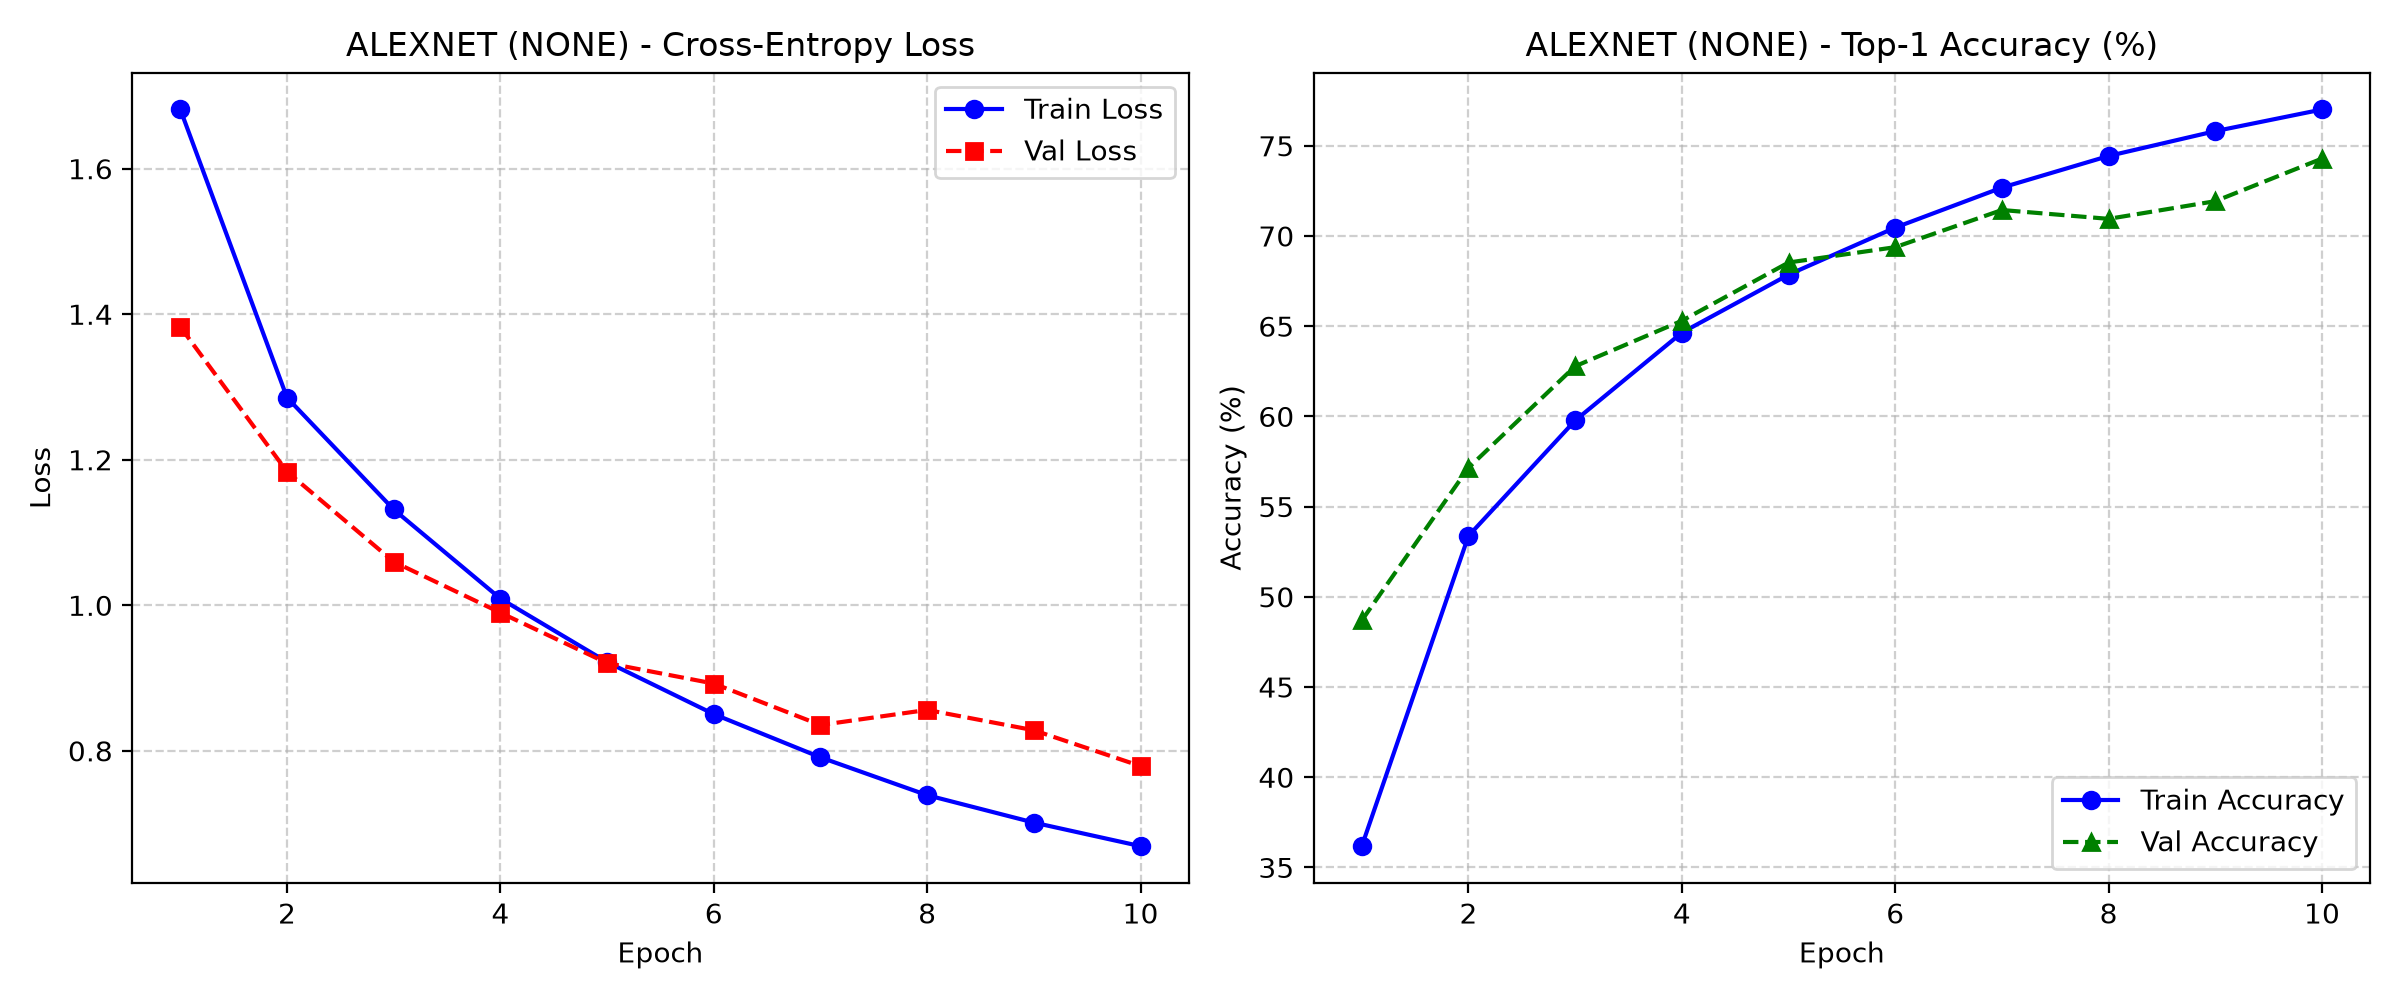
\includegraphics[width=\wfig]{plots/loss_alexnet_none.png}\\[2pt]
\includegraphics[width=\wfig]{plots/loss_alexnet_lrn.png}\\[2pt]
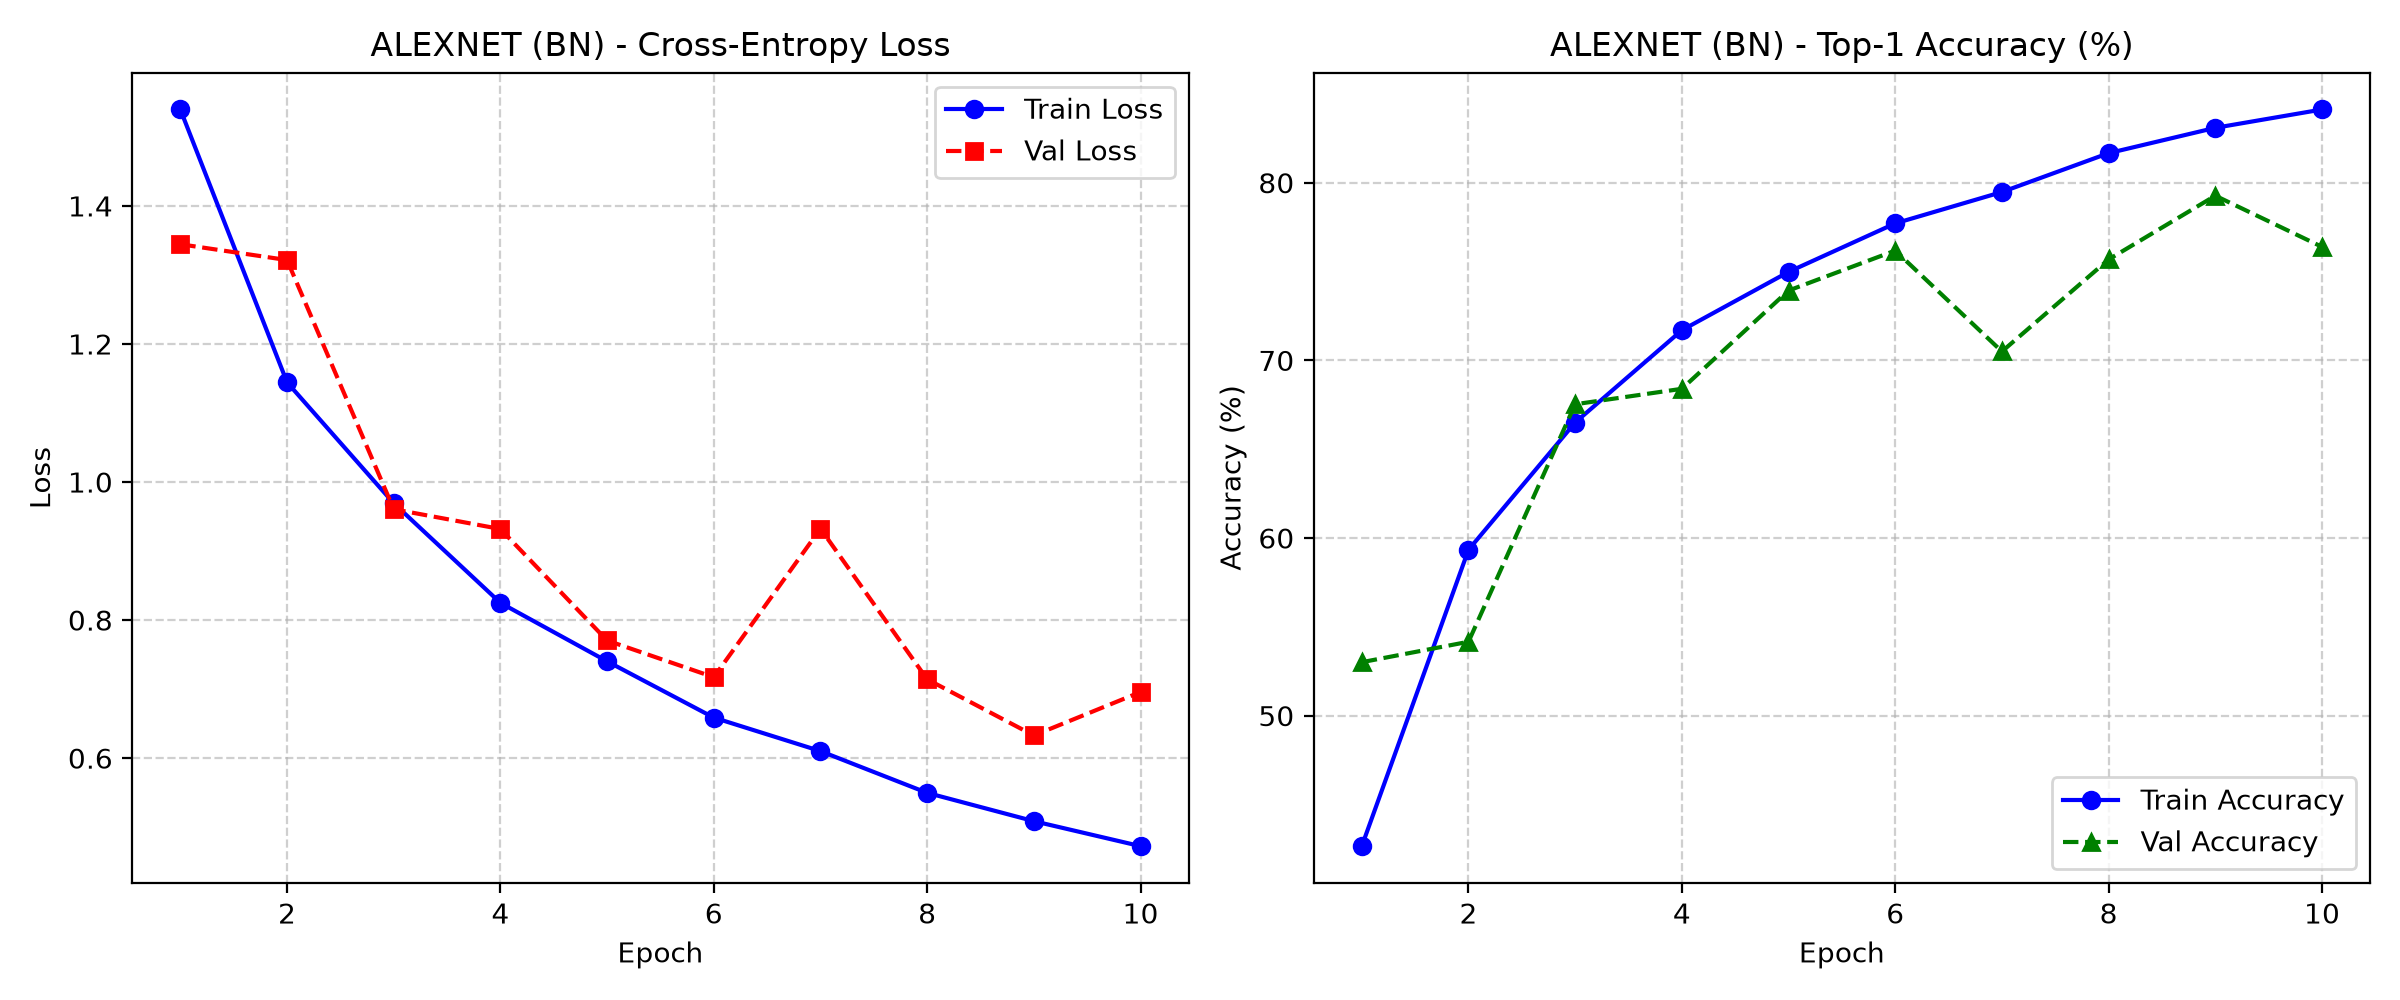
\includegraphics[width=\wfig]{plots/loss_alexnet_bn.png}
\caption{Normalization study, AlexNet-64 on CIFAR-10, 10 epochs, no augmentation: no normalization (top), LRN
(middle) and BatchNorm (bottom). All three use learning rate $10^{-3}$, batch size 128 and seed 42.}
\label{fig:norm}
\end{figure}

The extra cost of the normalization layers is small. The average epoch time on the T4 went from 23.9 s (no
normalization) to 25.0 s with BatchNorm (+4.6\%) and 26.3 s with LRN (+10\%). The profiler shows 437.17 MFLOPs for all
three versions, so it does not count the normalization layers. They are cheap next to the roughly 218.6 M
multiply-accumulates of the other layers, so the extra time probably comes from moving more data around. Running one
image at a time, the latency was 0.89 ms with no normalization, 0.90 ms with BatchNorm (+1\%) and 0.98 ms with LRN
(+10\%).

The training loss went down smoothly for all three versions. The validation curve of BatchNorm was the bumpiest, though:
at epoch 6 the validation loss jumped from 0.77 to 0.92 and the accuracy dropped from 73.8\% to 68.8\%, and then it
recovered. This is a single run, so we cannot say that BatchNorm is less stable in general. One possible reason is that
the batch statistics used in training are not exactly the same as the running statistics used for validation.

We repeated the BatchNorm run with seeds 42, 1 and 2 (Table~\ref{tab:seeds}) and got $79.36 \pm 1.07\%$ accuracy and
$79.27 \pm 1.34\%$ Macro-$F_1$, with single runs between 78.12\% and 80.02\%. The 6.4 and 4.8 point gaps are several
times bigger than this spread. The no-normalization and LRN results are from one seed each, so we do not know how much
they vary.

\subsection{Data Augmentation and the Generalization Gap}

Without augmentation, AlexNet + BatchNorm reached 90.31\% training accuracy but only 78.59\% validation accuracy at
epoch 15, a gap of $\Delta = 11.72$ points. Its validation loss was lowest at epoch 11 (0.59) and then went up to 0.72
while the training loss kept going down, which is what overfitting looks like. With augmentation, the gap at epoch 15
shrank to 2.99 points (84.64\% training and 81.65\% validation). The best validation accuracy went from 81.18\% to
82.83\% (+1.65 points), the best Macro-$F_1$ from 81.08\% to 82.90\%, and the final validation loss from 0.71 to 0.52
(Table~\ref{tab:aug} and Figure~\ref{fig:aug}).

Random crops, flips and colour changes do not change what is in the picture, but they show the network a slightly
different version of each image every epoch. This makes it harder to memorize exact pixel positions, so the network has
to use features that still work after a shift, a flip or a small colour change.

\begin{figure}[H]
\centering
\includegraphics[width=\wfig]{plots/loss_no_aug.png}\\[2pt]
\includegraphics[width=\wfig]{plots/loss_with_aug.png}
\caption{Augmentation study, AlexNet-64 + BatchNorm on CIFAR-10, 15 epochs: without augmentation (top) and with
augmentation (bottom).}
\label{fig:aug}
\end{figure}

Two things should be kept in mind. First, the spread between seeds that we measured (about 1 point) is similar to the
1.65-point gain in best accuracy, and each augmentation setting was run once, so the accuracy gain alone is not strong
evidence. The much smaller gap and the lower final validation loss are better evidence. Second, the training accuracy
with augmentation is measured on the augmented images, which are harder, so part of the smaller gap just comes from a
lower training accuracy. Augmentation also doubled the epoch time (about 52.9 s compared with 25.0 s), because the
transforms run on the CPU while the GPU waits. This comes from how our data loading is set up, not from the model.

\subsection{Learning Rate and Batch Size}

Table~\ref{tab:ablation} changes the learning rate and the batch size of the BatchNorm baseline (79.93\%). Every setting
was run once, and the baseline changes by about 1.1 points between seeds, so only the big differences mean something.

A learning rate of $10^{-4}$ gave 81.00\% (+1.07 points) and a higher training accuracy (89.9\% compared with 84.9\% at
epoch 10), but the accuracy difference is inside the seed spread. Batch size 32 (78.97\%, $-0.96$) is also inside it,
although each epoch took 32\% longer (33.0 s compared with 25.0 s) because there are four times as many steps. Batch
size 512 (77.69\%, $-2.24$) is a bit lower. It only makes 97 updates per epoch, which may be the reason, but we did not
test that.

The learning rate of $10^{-2}$ made a big difference (Figure~\ref{fig:lr}). With BatchNorm the network still trained,
but badly: it stayed at chance for the first two epochs, reached a best of 50.55\% and then became unstable at epoch 10
(44.79\%). Without normalization the training blew up: the training loss was 37.5 in epoch 1 and 66.3 in epoch 6, and
from epoch 2 on the validation accuracy stayed at 10.00\% with a Macro-$F_1$ of 1.82\%, which is what we get when the
network predicts one class for every image. So BatchNorm made the high learning rate usable in the sense that the
training did not collapse, but the results were still much worse than with $10^{-3}$ or $10^{-4}$ in 10 epochs. The
collapse without normalization looks similar to what happened to the Zoo AlexNet on Tiny ImageNet, which may be the same
kind of problem, but we did not check.

\begin{figure}[H]
\centering
\includegraphics[width=\wfig]{plots/loss_abl_bn_lr1e-2.png}\\[2pt]
\includegraphics[width=\wfig]{plots/loss_abl_none_lr1e-2.png}
\caption{Learning rate $10^{-2}$ on CIFAR-10, 10 epochs: with BatchNorm (top) and without normalization (bottom). The
titles of the plots do not show the learning rate.}
\label{fig:lr}
\end{figure}

\subsection{Tiny ImageNet}

AlexNet-64 with BatchNorm reached 28.31\% accuracy and 26.99\% Macro-$F_1$ on the official validation images after 10
epochs (Table~\ref{tab:perf}). That is about 57 times better than random guessing (0.5\% for 200 classes), so it did
learn useful features, but it is far below the 80--83\% on CIFAR-10. Tiny ImageNet is harder because it has 200
detailed classes instead of 10, only 500 training images per class instead of 5{,}000, and more varied objects at the
same $64{\times}64$ size.

The LeNets show the same pattern as on CIFAR-10: the modernized LeNet gets 19.10\% compared with 9.84\% for the base
LeNet (+9.3 points, compared with +11.1 points on CIFAR-10). Macro-$F_1$ is lower than accuracy for every model (26.99\%
compared with 28.31\% for AlexNet) even though every class has 50 validation images, so some classes work better than
others.

\begin{figure}[H]
\centering
\includegraphics[width=\wfig]{plots/loss_tiny_imagenet.png}\\[2pt]
\includegraphics[width=\wfig]{plots/loss_zoo_alexnet_tiny.png}
\caption{Tiny ImageNet: AlexNet-64 + BatchNorm (top) and the Zoo AlexNet (bottom). The ``validation'' curves in these
plots use the training images, see Section~\ref{sec:setup}. The axes of the bottom plot are zoomed in a lot (the loss only changes in
the fourth decimal place), so the Zoo run is flat at chance and not noisy.}
\label{fig:tiny}
\end{figure}

The scores on the official validation images were only 1 to 3 points below the accuracy measured on the training images
(28.31\% compared with 31.65\% for AlexNet). So after 5 to 10 epochs the models were still underfitting, not
overfitting. The curves in Figures~\ref{fig:tiny} and~\ref{fig:lenettiny} use the training images as the validation
set, so they cannot show overfitting, but the loss kept going down until epoch 10 (from 4.34 to 2.90 for AlexNet). The
loss on the official validation images was 3.08.

\begin{figure}[H]
\centering
\includegraphics[width=\wfig]{plots/loss_lenet_tiny.png}\\[2pt]
\includegraphics[width=\wfig]{plots/loss_lenet_modern_tiny.png}
\caption{Tiny ImageNet, 5 epochs: base LeNet-5 (top) and modernized LeNet (bottom). As in
Figure~\ref{fig:tiny}, the ``validation'' curves use the training images.}
\label{fig:lenettiny}
\end{figure}

\subsection{Model Zoo AlexNet}

On CIFAR-10 (10 epochs, no augmentation, no normalization) the Zoo AlexNet reached 64.37\% accuracy and 64.19\%
Macro-$F_1$. That is 9.2 points lower than AlexNet-64 without normalization (73.52\% / 73.48\%), even though it has 8.6
times more parameters (57.04 M compared with 6.61 M). It uses fewer FLOPs on $64{\times}64$ input (188.3 M compared with
437.2 M) but has a longer epoch (29.4 s compared with 23.9 s) and a higher latency (1.79 ms compared with 0.89 ms). A
likely reason is that the network was designed for $224{\times}224$ images. The $11{\times}11$ stride-4 convolution and
the pooling layers shrink a $64{\times}64$ image to a $1{\times}1$ map, so the convolution layers do little work, and
the input to the linear layers is the same 256 numbers copied 36 times. About 66\% of the parameters are in a layer that
gets no extra spatial detail. We did not test this explanation. The validation accuracy also dropped in the last epoch
(64.37\% to 62.98\%), so this run had not settled yet.

On Tiny ImageNet the Zoo AlexNet did not learn with learning rate $10^{-3}$: the accuracy stayed at the chance level of
0.50\%, the Macro-$F_1$ was 0.00 and the loss stayed at about 5.299, which is almost exactly $\ln 200 = 5.298$, the
loss of a network that gives the same answer for every image. The same network did learn on CIFAR-10 (64.37\%), so we
think the large network without normalization was unstable at this learning rate, but we did not check the cause.

\end{document}
